\section{Thursday, August 31, 2023}
\subsection{Logical Equivalence}
In logic, when we say that two statements show the same T/F value for every possible combination of component statement variables, we like to consider those two statements \vocab{logically equivalent}. This is commonly denoted through the "\equiv" symbol.

\begin{example}
    Is the following logically equivalent? \(p\) and \neg{(\neg{p})}
\end{example}

This example is very, very elementary, but let's just show it through a truth table in case you're scratching your head at it.

\begin{displaymath}
    \begin{array}{|c|c|c|}
    p & \neg{p} & \neg{(\neg{p})}\\ 
    \hline
    T & F & T\\
    F & T & F\\
    \end{array}
\end{displaymath}

Through this truth table, now we see that the first column is directly equivalent to the last column for any value, so: \(p\) \equiv \neg{(\neg{p})}.

This is considered the \vocab{double negative}.

\subsection{DeMorgan's Laws}
In logical equivalence, there are two laws that will be extensively used called \vocab{DeMorgan's laws}. These cover two very important logical equivalencies.

\begin{displaymath}
    \neg{(p \lor q)}\equiv \neg{p} \land \neg{q}
\end{displaymath}

\begin{displaymath}
    \neg{(p \land q)}\equiv \neg{p} \lor \neg{q}
\end{displaymath}
 
We can use these two laws when we prove logical equivalency to hasten our final conclusion.

\subsection{Tautologies and Contradictions}
\vocab{Tautologies} are a form of statement in which the statement form is \textbf{true} for all values, no matter true nor false.

Say for example, we have \(x\) as a tautology. Therefore, we can simply write:

\begin{displaymath}
    x = t
\end{displaymath}

\begin{example}
    An elementary tautology is $p \land \neg{p}$.
\end{example}

\vocab{Contradictions}, on the other hand, are a form of statement in which the statement form is \textbf{false} for all values, no matter true nor false.

Say for example, we now have \(y\) being a contradiction. Therefore, we can simply write:

\begin{displaymath}
    y = c
\end{displaymath}

\begin{example}
    An elementary contradiction is $p \lor \neg{p}$.
\end{example}

\subsection{Condensing and Proving Logical Equivalencies}
Over time, many particular logical equivalencies have been created, to a point where we can consider them as generalized laws that we may use to help in our steps to prove logical equivalencies that have not been proven. We call these the \vocab{common logical equivalencies} as demonstrated in the table below.

\vspace{0in}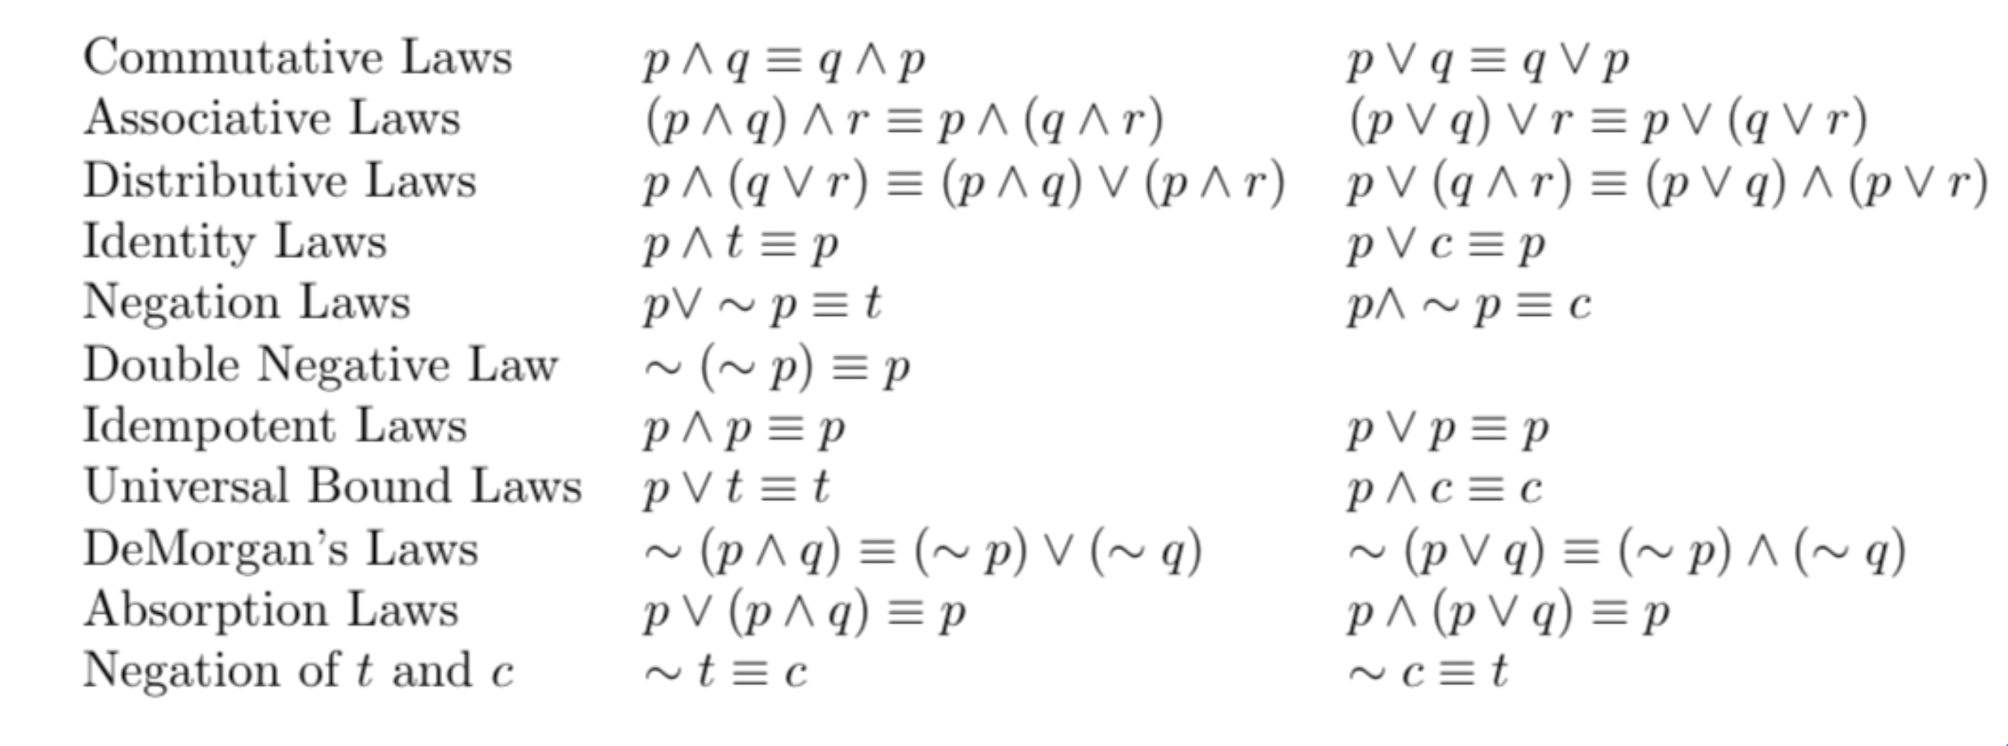
\includegraphics[scale=0.4]{media/commonlogicalequivalencies.png} \\

Lets use these laws to prove some logical equivalencies ourselves.

\begin{example}
    Prove $\neg(\neg p\land q)\land(p\lor q)\equiv p.$
\end{example}

Using the table above, this would be the proof (there can be other solutions!) to this example.
\begin{logicproof}{1}
    \neg{(\neg{p}\land q)\land(p\lor q)} & Original Left Side \\
    (\neg({\neg{p})}\lor \neg{q})\land (p\lor q) & DeMorgan's Law \\
    (p\lor \neg{q}) \land (p\lor q) & Double Negative Law \\
    p \lor (\neg{q}\land q) & Distributive Law \\
    p \lor c & Negation Law \\
    p & Identity Law
\end{logicproof}

\subsection{Conditional Statements}
In logic, we can also consider implications of statements such like "if \(p\), then \(q\)." These are considered \vocab{conditional statements}, and they too can be treated as ordinary logic signs (there is also a logical equivalency for implications and normal logic signs).

Say we have statement variables \(p\) and \(q\). We can then derive a conditional form:

\begin{displaymath}
    p \rightarrow q
\end{displaymath}

The general idea for implication is that if we have \(p\) being true and \(q\) being false, then the implication is then false. However, otherwise the implication is always true.

The logical equivalence of the normal conditional is:

\begin{displaymath}
    p \rightarrow q \equiv \neg p \lor q
\end{displaymath}

This can be written in logical equivalence proofs by just indicating that this is the "definition of implication" or "definition of conditional."